% Gemini theme
% https://github.com/anishathalye/gemini

\documentclass[final]{beamer}

% ====================
% Packages
% ====================

\usepackage[T1]{fontenc}
\usepackage{lmodern}
\usepackage[size=custom,width=120,height=72,scale=1.0]{beamerposter}
\usetheme{gemini}
%\usecolortheme{mit}
\usecolortheme{gemini}
\usepackage{graphicx}
\usepackage{booktabs}
\usepackage{tikz}
\usepackage{pgfplots}
\usepackage{pgf}
%\usepackage{cmbright}
\usepackage{wrapfig}
%\usepackage{balance}
%\usepackage{siunitx}
\usepackage{dcolumn}
  \newcolumntype{d}[1]{D{.}{.}{#1}}
  \newcommand\mc[1]{\multicolumn{1}{c}{#1}} % handy shortcut macro
\usepackage{gensymb}
% Center captions
\usepackage[center]{caption}

%% Bibliography
%\usepackage[utf8]{inputenc}
%\usepackage[english]{babel}
%\usepackage{biblatex}
\usepackage[backend=biber, style=numeric]{biblatex}
\AtBeginBibliography{\small}
%\usepackage[backend=biber, style=authoryear, doi=false,isbn=false,url=false, giveninits=true]{biblatex}
\addbibresource{poster.bib}

% ====================
% Additional Config
% ====================

\graphicspath{ {images/} }
%\renewcommand{\thefootnote}{\arabic{footnote}}
%\renewcommand{\thefootnote}{\fnsymbol{footnote}}

%% % Allow footnotes to play nice with beamer
%% \addtobeamertemplate{footnote}{\vspace{-6pt}\advance\hsize-0.5cm}{\vspace{6pt}}
%% \makeatletter
%% % Alternative A: footnote rule
%% \renewcommand*{\footnoterule}{\kern -3pt \hrule \@width 2in \kern 8.6pt}
%% % Alternative B: no footnote rule
%% % \renewcommand*{\footnoterule}{\kern 6pt}
%% \makeatother

% ====================
% Lengths
% ====================

% If you have N columns, choose \sepwidth and \colwidth such that
% (N+1)*\sepwidth + N*\colwidth = \paperwidth
\newlength{\sepwidth}
\newlength{\colwidth}
% 3 Columns
%\setlength{\sepwidth}{0.025\paperwidth}
%\setlength{\colwidth}{0.3\paperwidth}
% 4 Columns
\setlength{\sepwidth}{0.025\paperwidth}
\setlength{\colwidth}{0.21875\paperwidth}

\newcommand{\separatorcolumn}{\begin{column}{\sepwidth}\end{column}}

% ====================
% Title
% ====================

\title{Eclipsing Binary RZ Cassiopeiae: Generating a light curve with a DSLR camera}

\author{Sam Nelson}
%\author{Sam Nelson \inst{1}}

%\institute[shortinst]{\inst{1} Boise State University}
\institute[shortinst]{Boise State University}

% ====================
% Footer (optional)
% ====================

\footercontent{
  \href{https://www.boisestate.edu/physics/}{https://www.boisestate.edu/physics/} \hfill
  Physics 205 - Stellar Astronomy --- Class Project \hfill
  \href{mailto:samnelson@u.boisestate.edu}{samnelson@u.boisestate.edu}}
% (can be left out to remove footer)

% ====================
% Logo (optional)
% ====================

% https://www.boisestate.edu/communicationsandmarketing/brand-standards/logos/
% https://www.boisestate.edu/licensing/trademarks/logo-artsheet/

% use this to include logos on the left and/or right side of the header:
\logoright{
\includegraphics[height=7cm]{blue_bsu_logo.pdf}}
% \logoleft{\includegraphics[height=7cm]{logo2.pdf}}

% ====================
% Body
% ====================

\begin{document}

\begin{frame}[t]
\begin{columns}[t]
\separatorcolumn

\begin{column}{\colwidth}
  \begin{block}{Introduction}
    Photometry is the process of measuring the intensity of light. It doesn't
    sound particularly glamorous, but it is an extremely important tool used
    by astronomers to study remote astronomical objects.

    One area of study is the observation of variable stars, including eclipsing
    binary stars. I wanted to use this project as an opportunity to learn more
    about the technique of photometry. I was also curious as to the quality of
    data that could be gathered by the amateur astronomer with a relatively cheap
    consumer DSLR camera and lens.
  \end{block}

  \begin{block}{Selecting a target: RZ Cassiopeiae}
    While I have done some astronomical observing before, this was the first time I 
    had dabbled in photometry or astrophotography. Because of this, I wanted a target which
    was easy to observe. After consulting the American Association of Variable Star Observers (AAVSO)
    beginner guides and other resources on the web, I chose RZ Cas, an Algol type
    eclipsing binary.

    RZ Cas has some characteristics which make it a very good target for beginners:

    \begin{itemize}
      \item \textbf{Period:} The primary eclipse repeats every 1.195258 days ($\sim$28.7hrs)
      \item \textbf{Magnitude Range:} The magnitude ranges from $\sim$6.2 to $\sim$7.6
      \item \textbf{Eclipse Length:} The primary eclipse lasts just under 5hrs
      \item \textbf{Location:} RZ Cas is located at +69$\degree$, circumpolar for our latitude
      \item \textbf{Comparison:} Suitable comparison stars are located within a few degrees
    \end{itemize}

    This made it possible for me to observe the primary eclipse in one evening. If 
    problems arose with weather, another observing opportunity would be available in 
    a few days.

    Due to light pollution at my observing location, the target star was not visible 
    with the naked eye. However, it was visible in binoculars, and as the following
    finder chart shows, easy to visually "starhop" to from the familiar \textbf{W} asterism
    in Cassiopeia.

    \begin{figure}
      \centering
      \resizebox{.9\linewidth}{!}{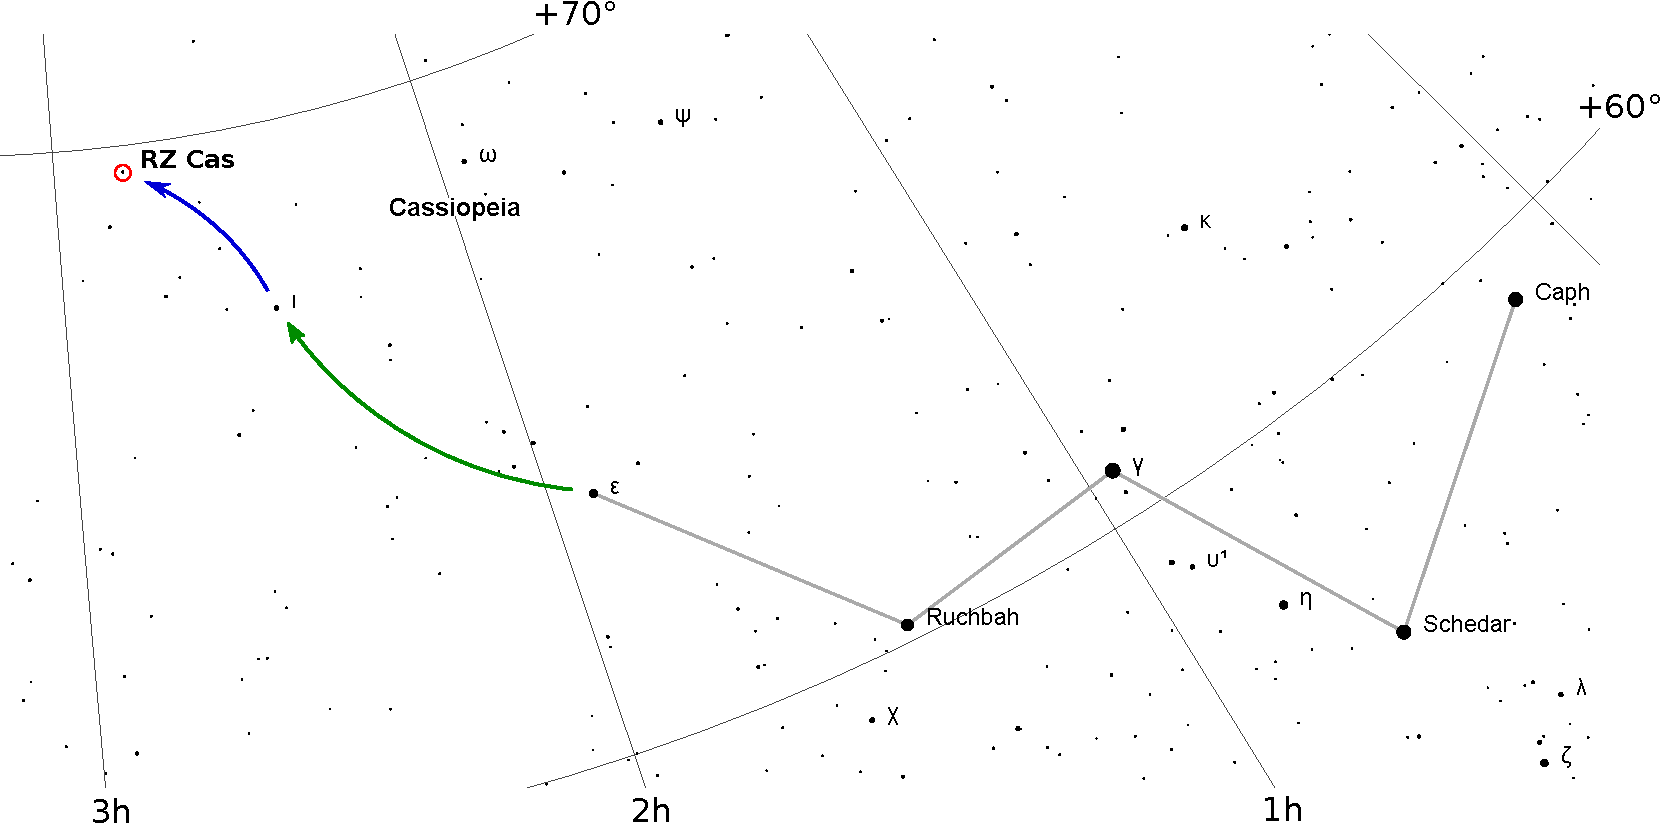
\includegraphics{figs/finder_chart/RZ_Cas_Finder_Chart.pdf}}
      \caption{RZ Cas finder chart}
    \end{figure}
  \end{block}


\end{column}

\separatorcolumn

\begin{column}{\colwidth}

  \begin{block}{Observation}
    \begin{wrapfigure}{R}{0.4\textwidth}
      \centering
      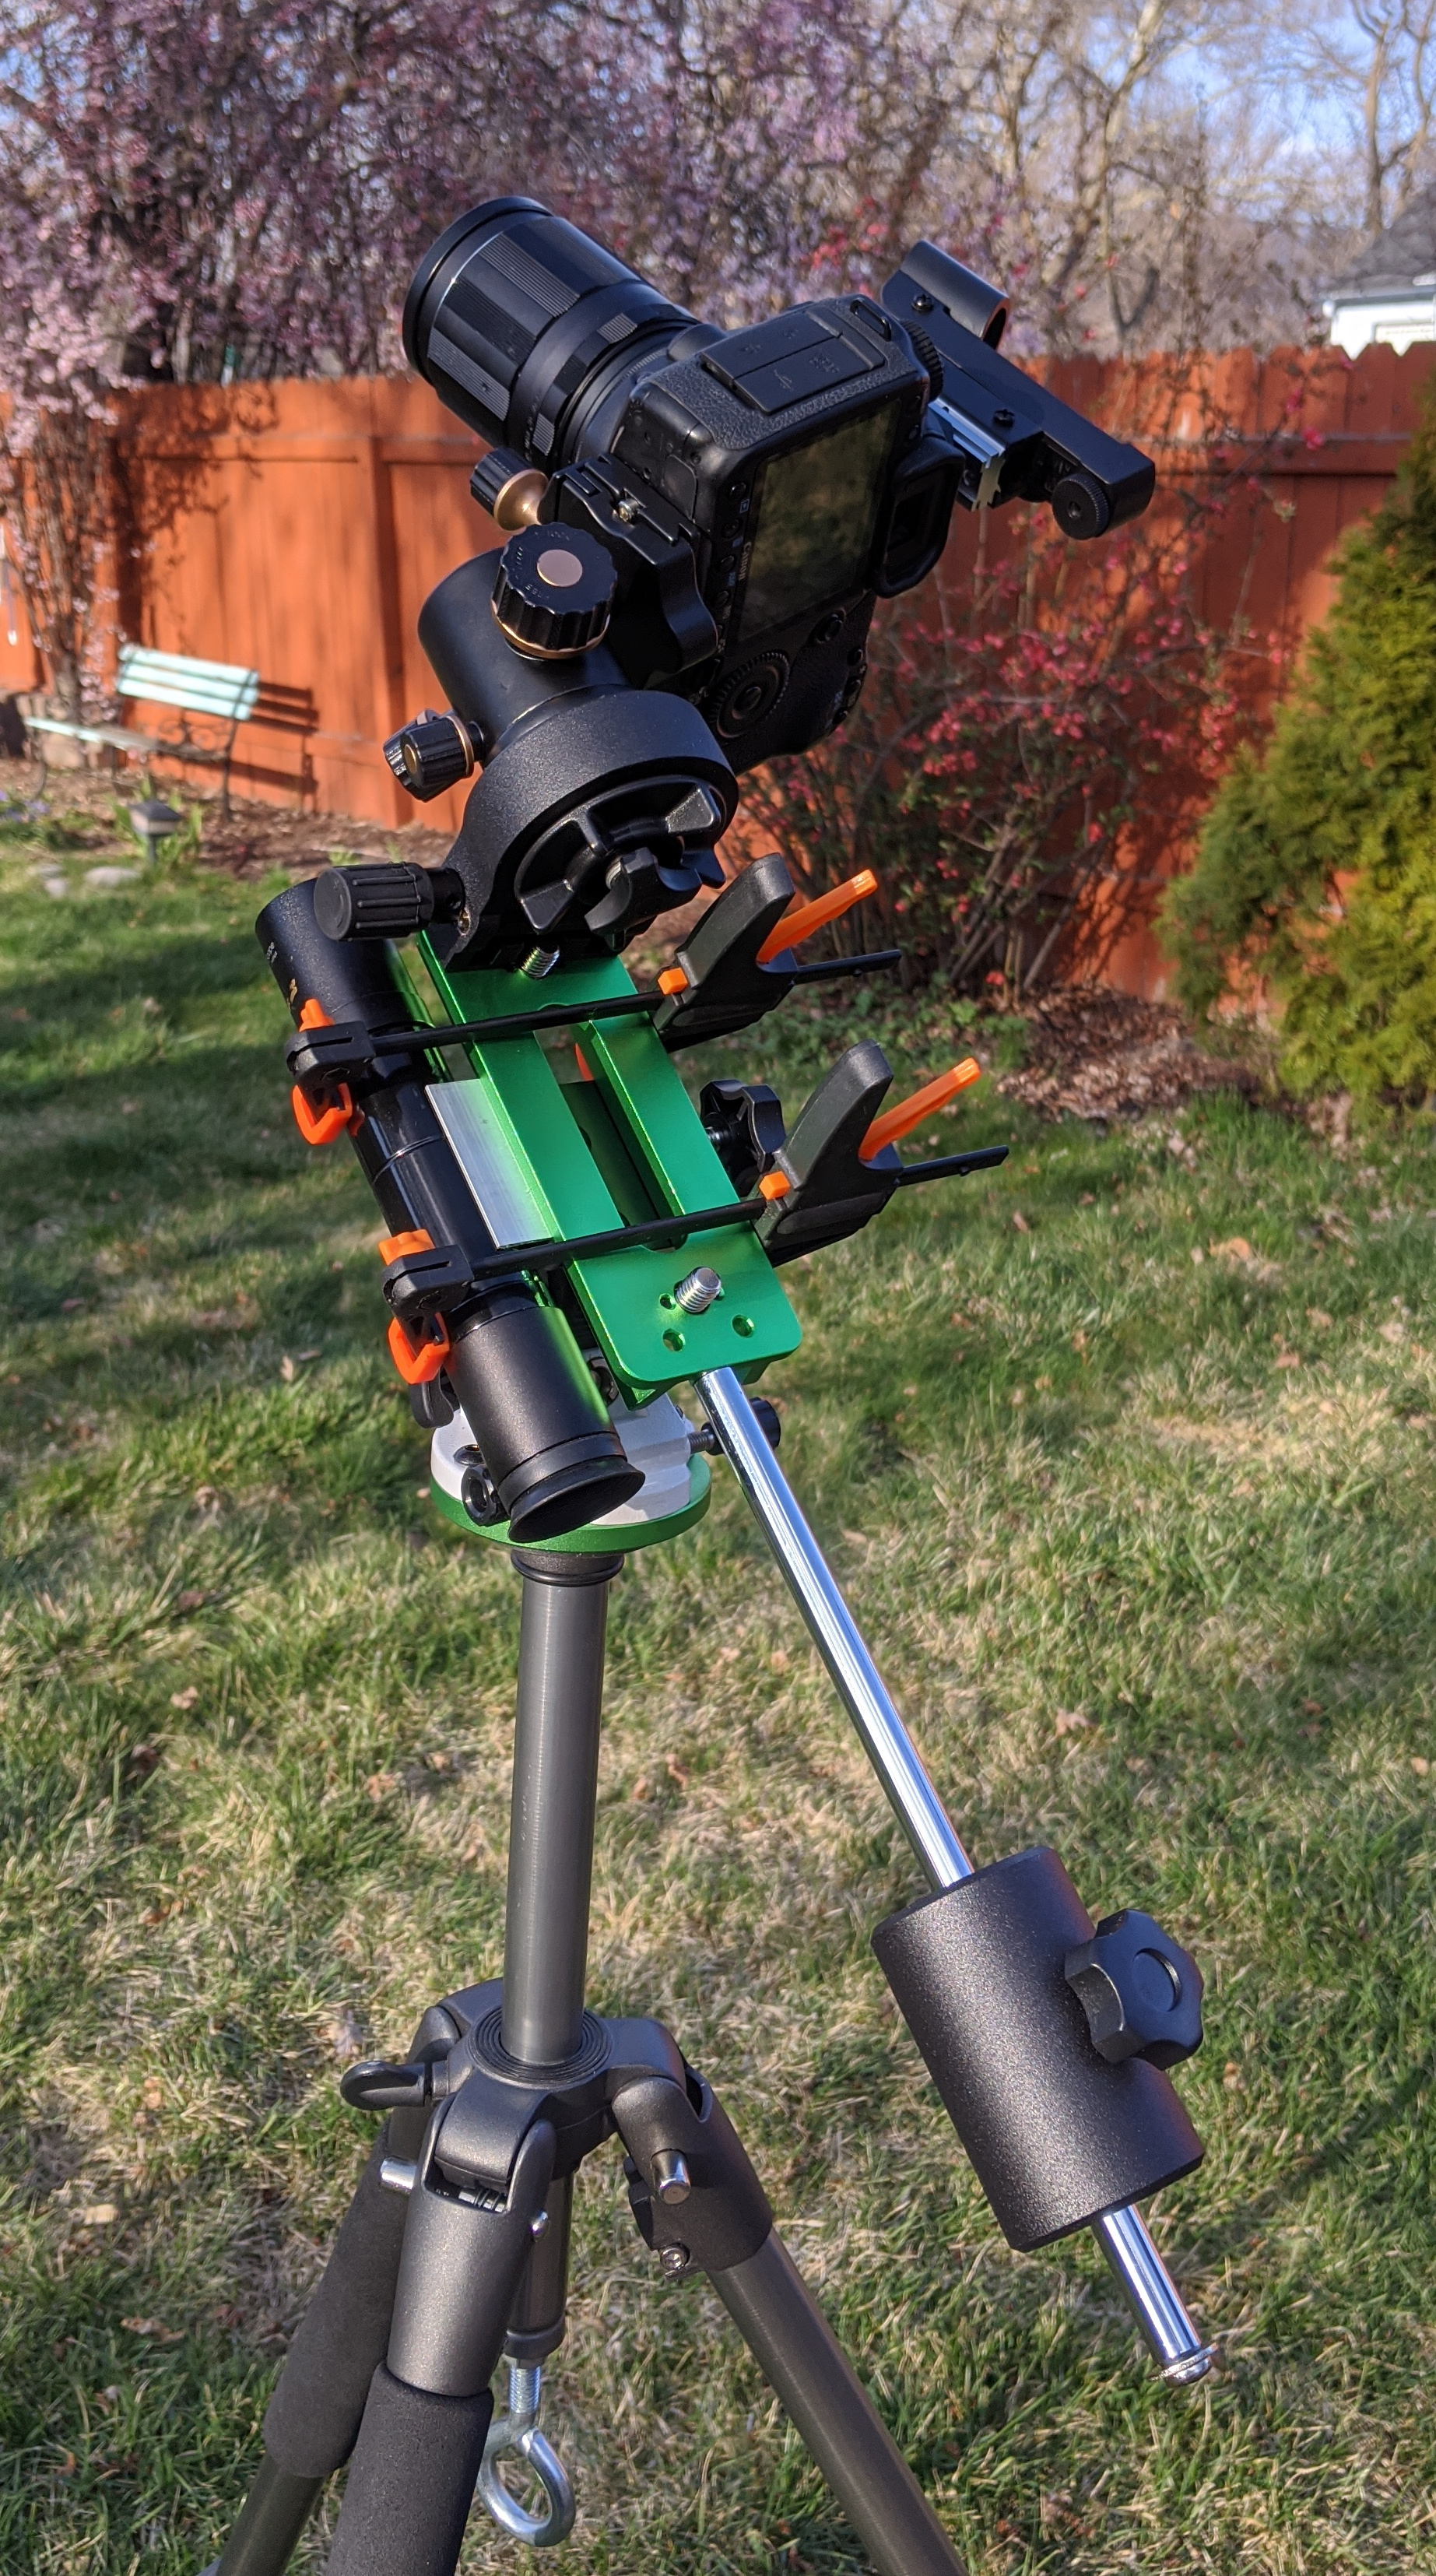
\includegraphics[width=0.35\textwidth]{camera_and_mount-crop.jpg}
      \caption{DSLR camera and cobbled together mounting hardware}
    \end{wrapfigure}

%    I originally planned to observe using my ancient Canon EOS300D DSLR camera with
%    a 50mm lens. The goal was to keep the cost of the project very low.  Initial testing 
%    showed that while this equipment would work, it had some frustrating limitations. 
%
%    To keep the low cost goal, the camera was replaced with a \$75 Canon EOS40D from Ebay
%    and a \$100 135mm telephoto lens originally meant for a 1970's vintage Pentax film 
%    camera. With the addition of a red-dot finder scope and a few other Ebay sourced parts,
%    this combination proved to work very well and without most of the frustrations
%    of the original equipment.

    A Canon EOS40D DSLR with a 135mm telephoto lens was used. This resulted
    in a field of view of $\sim$9$\degree$. Originally a 50mm lens was used but the wide
    field of view made placing photometric apertures more difficult.  A polar finder scope was clamped along the axis of the manual RA adjustment mount. The scope was used to roughly align the axis with the celestial north pole near Polaris. 
%    This allowed the camera to rotate as the earth turned and kept the orientation of the photographs
%    relatively constant during the observing session.

    Conditions were cold (25$\degree$F) and clear during the evening. However, there was some 
    cloud cover for over an hour during the midpoint of the eclipse. The camera and mount 
    also had to be moved twice as the target star moved behind trees and other obstacles.  
    Eclipse timing predictions are available online and were used to pick the observation 
    time.
%    time for observations. The predicted start time was at 11:11pm MDT. 
%      The measured light curve is not accurate to the minute but you can see a noticeable dip approximately 10 minutes after 11pm.
    % Eclipse timing?

  \end{block}

  \begin{block}{Star Field}
%    Even though I suspected that I had missed the eclipse minimum due to cloud cover, the
%    data that was gathered looked very promising. I could visually see the star dimming
%    through binoculars and the dimming was even more obvious in the photographs.

    Sets of 20 images with exposure time of 10s each were taken approximately every ten
    minutes. These 20 images were subsequently calibrated using Dark, Flat and Bias frames
    to correct for camera noise, lens distortion and dust/defects. Calibrated images were
    then aligned and stacked by averaging. A annotated example of a fully processed image
    is below. The target, RZ Cas is visible near the center of the image.

    \begin{figure}
      \centering
      \resizebox{.9\linewidth}{!}{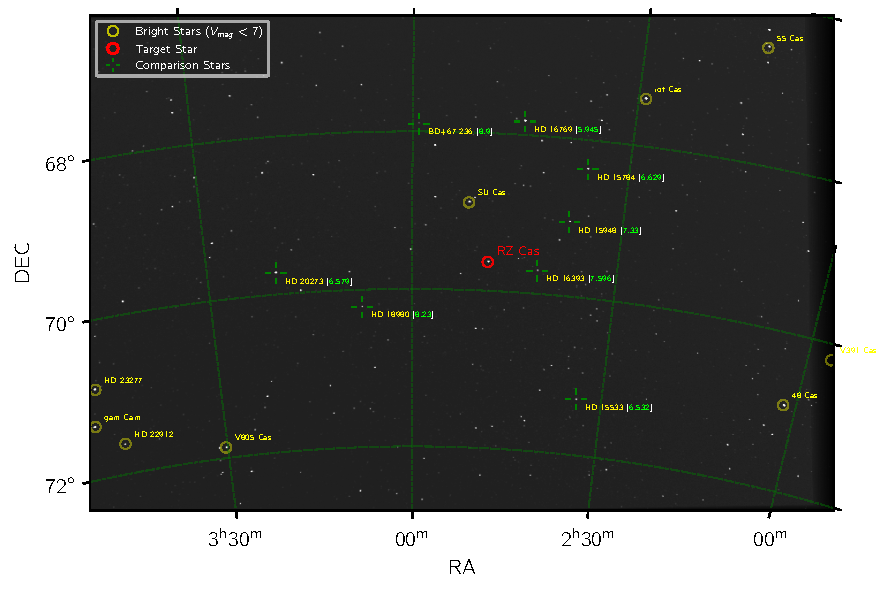
\includegraphics{figs/star_field/RZCas_star_field.pdf}}
        \caption{RZ Cas star field (stacked image), annotation data from \cite{2000A&AS..143....9W}}
    \end{figure}

  \end{block}

\end{column}

\separatorcolumn

\begin{column}{\colwidth}

  \begin{block}{Photometry}
    Rather than doing differential photometry against a single comparison star, 8 stars
    were chosen. This process is known as \textit{Ensemble Photometry}. This minimizes 
    errors from individual stars. At its lowest point during the night, RZ Cas was 
%    $43\degree - (90\degree - 69\degree) \approx 22\degree$ above the northern horizon.
    $\sim22\degree$ above the northern horizon.
    Atmospheric effects are pronounced this close to the horizon and multiple comparison
    stars are one way to help to mitigate these effects.

    Following is the list of the photometry comparison stars used to compute the 
    relative magnitude of the target in each frame. Note that the Johnson V magnitudes 
    of the list of stars encompass the full expected range of magnitude of RZ Cas 
    during the eclipse ($\sim$6.2 to $\sim$7.6). This ensures that the magnitude 
    values can be \textit{interpolated} rather than \textit{extrapolated}. 
    \textit{AstroimageJ} was used to perform photometry.

    \begin{table}
      \setlength{\tabcolsep}{1em} % for the horizontal padding
      \centering
        \begin{tabular}{l c c *{1}{d{4.3}} }
        \toprule
          \mc{\textbf{Name}} & \mc{\textbf{RA}} & \mc{\textbf{DEC}} & \mc{\textbf{Mag V}} \\
        \midrule
          HD 16769  & 02:44:52.806 & +67:49:47.54 & 5.945 \\
          HD 15533  & 02:34:00.550 & +71:17:23.15 & 6.532 \\
          HD 20273  & 03:19:59.417 & +69:43:41.31 & 6.579 \\
          HD 15784  & 02:35:45.859 & +68:22:16.00 & 6.629 \\
          HD 15948  & 02:37:35.107 & +69:03:28.63 & 7.33  \\
          HD 16393  & 02:41:36.217 & +69:42:28.92 & 7.596 \\
          HD 18980  & 03:07:30.003 & +70:13:04.80 & 8.23  \\
          BD+67 236 & 02:59:11.623 & +67:54:11.10 & 8.9   \\
        \bottomrule
      \end{tabular}
      \caption{Photometric comparison stars, from \cite{2000A&AS..143....9W}}
    \end{table}

  \end{block}

  \begin{block}{Light Curve Results}

    After all the preparation, finally we can see the data! Unfortunately,
    due to the intermittent cloud cover, the entire eclipse minimum was missed.
    A Gaussian curve fit was generated so that the general shape of the light 
    curve can be better seen.

    \begin{figure}
      \centering
        \resizebox{.9\linewidth}{!}{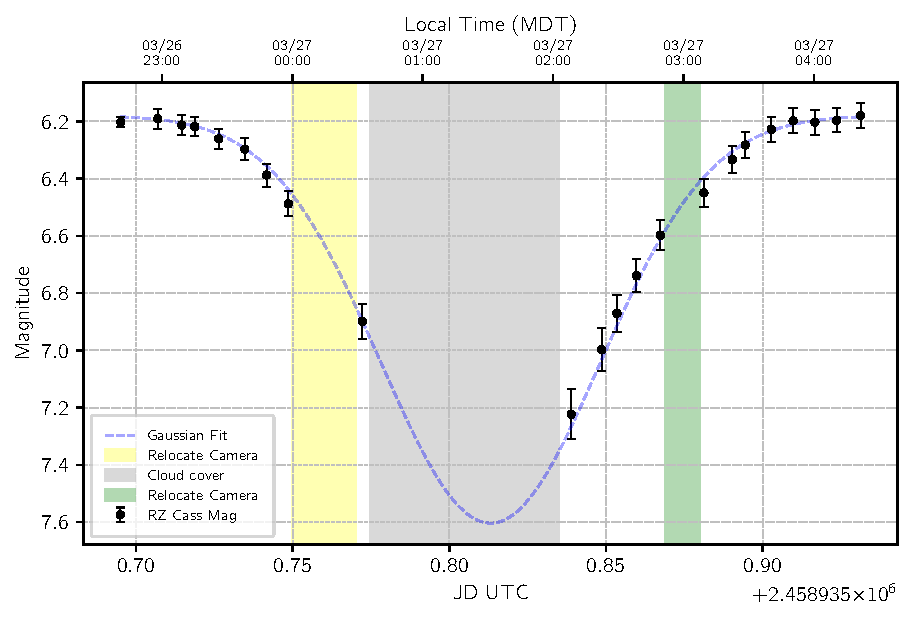
\includegraphics{figs/light_curve/RZCas_light_curve.pdf}}
      \caption{RZ Cas primary eclipse light curve}
    \end{figure}

  \end{block}

\end{column}

\separatorcolumn

\begin{column}{\colwidth}

  \begin{block}{Reference RZ Cas Light Curve}
    For comparison, here is a light curve for RZ Cas measured in the 1970's
    which shows not only the primary eclipse, but also the much smaller magnitude
    but still clearly visible secondary eclipse.

    \begin{figure}
      \centering
      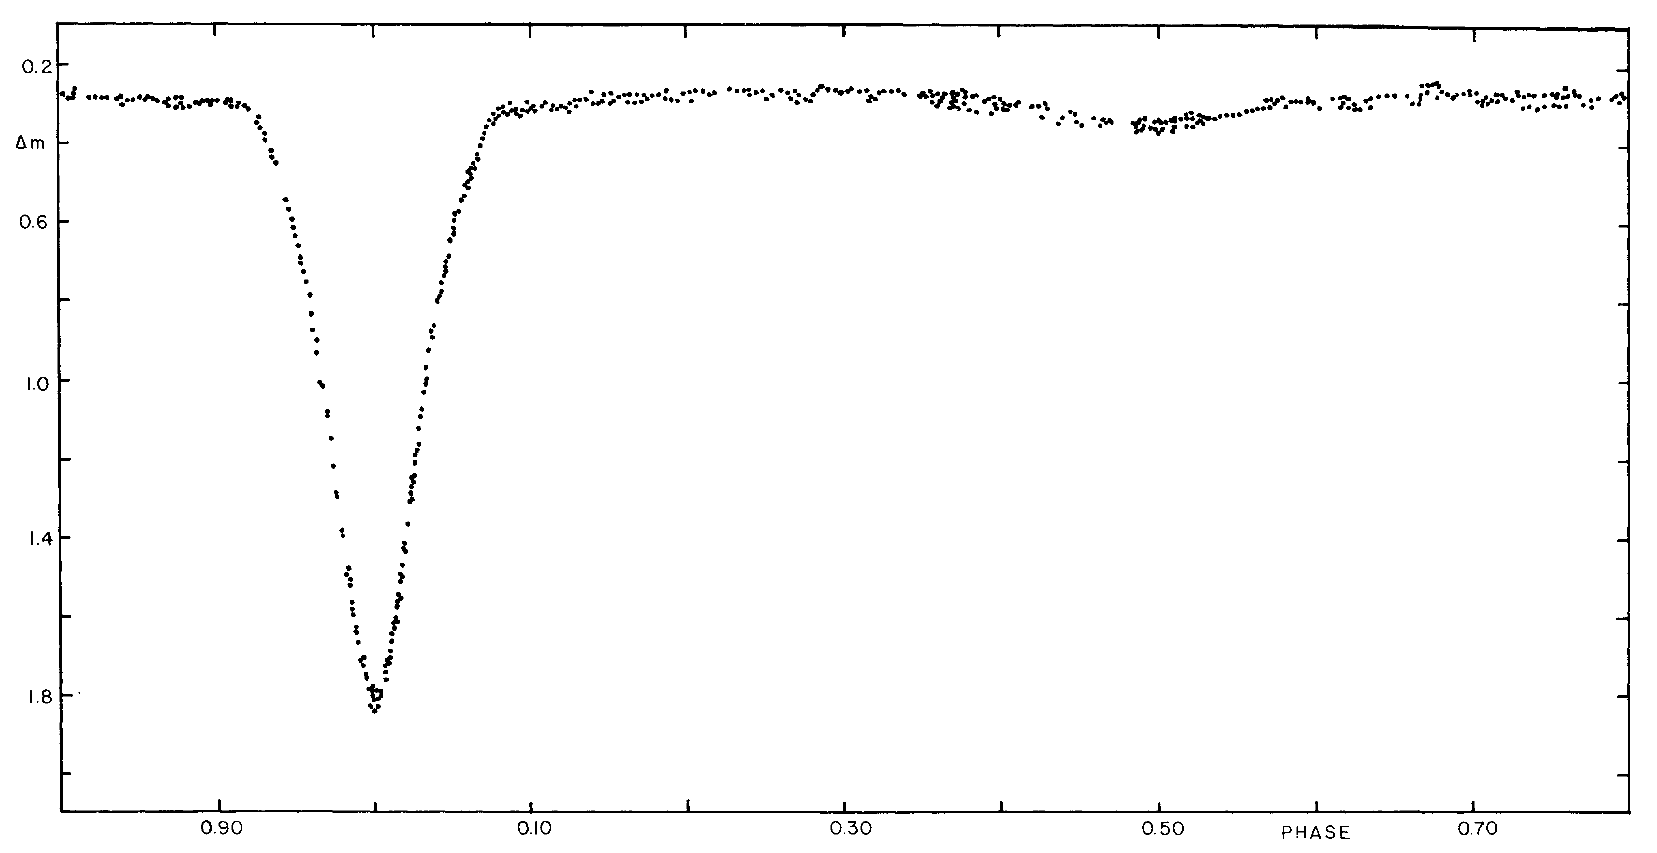
\includegraphics[width=0.9\textwidth]{Reference_RZ_Cas_Light_Curve.png}
        \caption{The light curve of RZ Cas in yellow light. The vertical scale plots \textbf{\Delta{m}} (RZ Cas - HR 791) \cite{Chambliss_1976}}
    \end{figure}

  \end{block}

  \begin{block}{Conclusion}
    Despite the incomplete results due to cloud cover during the observation
    session, I believe the project was a success. It demonstrated the practicality
    of using an affordable consumer DSLR camera and lens to gather useful photometric
    data.

    However, if I continue making photometric observations in this manner, I would make some
    changes. A star tracker would limit the need to make constant camera
    alignment checks. A better observing location free from major obstacles and excessive
    light pollution would improve the quality of results.
  \end{block}

  \begin{block}{References}

    % Show all bibliography entries regardless of citation
    \nocite{*}
    \printbibliography

  \end{block}

\end{column}

\separatorcolumn
\end{columns}
\end{frame}

\end{document}
